\documentclass{article}
\usepackage{amsmath}
\usepackage{amsfonts}
\usepackage{amssymb}
\usepackage{mathtools}
\usepackage{tcolorbox}
\usepackage[inline]{enumitem}
\usepackage[a4paper,margin=1in]{geometry}
\usepackage[normalem]{ulem}
\usepackage{graphicx}
\usepackage{tasks}
\settasks{label=(\alph*), label-offset=0.4em, label-width=1.5em}

\usepackage{fancyhdr}
\fancyhf{}
\setlength{\headheight}{36pt}
\renewcommand{\headrulewidth}{0pt}
\thispagestyle{fancy}
\lhead{Calculus Exercise}
\chead{Week 16 (10.3, 10.4)}
\rhead{\underline{ID:\hspace{7.4em}} \\ \vspace{0.2cm} \underline{Name:\hspace{6em}}}
\cfoot{\thepage}

\begin{document}
\begin{enumerate}
\item[10.3.52]
    Show that the curve $r=2- \csc\theta$ (a conchoid)  has the line $y=-1$
    as a horizontal asymptote by showing that
    $\displaystyle \lim_{r \longrightarrow \pm \infty} y = -1$. Use this fact to help
    sketch the conchoid.

\vspace{6cm}

\item[10.3.54]
    Sketch the curve $(x^{2}+y^{2})^{3}=4x^{2}y^{2}$.

\vspace{6cm}

\item[10.3.58]
    Show that the curves $r=a \sin\theta$ and $r = a \cos\theta$
    intersect at right angles.

\newpage

\item[10.4.10]
    Sketch the curve and find the area that it encloses.
    \[
        r = 2 + 2 \cos\theta
    \]

\vspace{8cm}

\item[10.4.28]
    Find the area of the region that lies inside the first curve
    and outside the second curve.
    \[
        r = 3\sin\theta,\ r = 2 - \sin\theta
    \]

\newpage

\item[10.4.45]
    Find the area of the shaded region.
    \begin{center}
        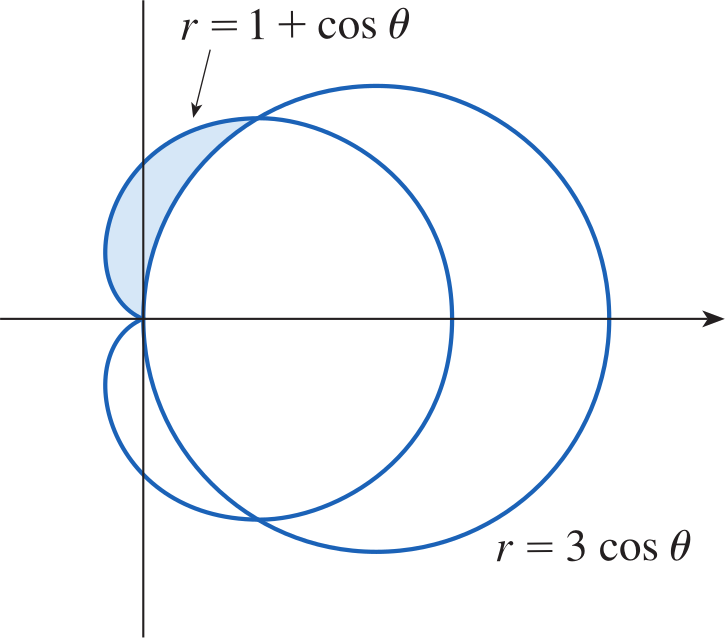
\includegraphics[height=5cm]{./png/10.4.45.png}
    \end{center}

\vspace{6cm}

\item[10.4.53]
    Find the exact length of the portion of the curves shown
    in blue.
    \begin{center}
        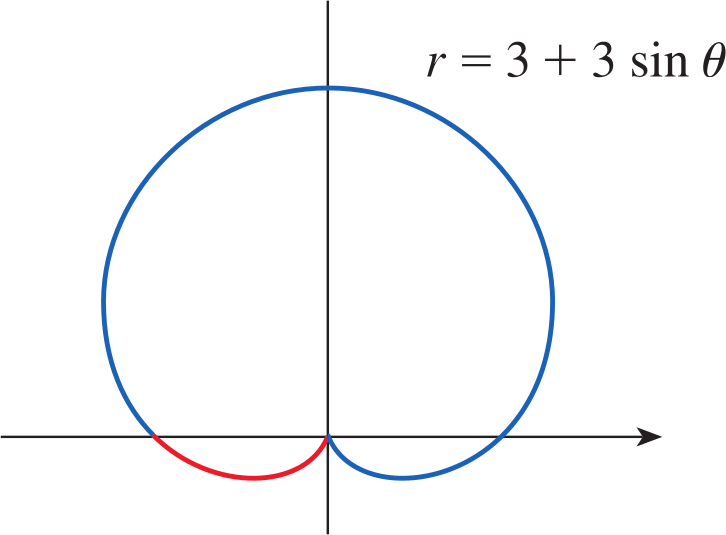
\includegraphics[height=5cm]{./png/10.4.53.png}
    \end{center}

\newpage

\item[10.4.68]
    Find the slope of the tangent line to the given polar
    curve at the point specified by the value of $\theta$.
    \[
        r = 1 + 2 \cos\theta,\ \theta = \pi/3
    \]

\end{enumerate}
\end{document}
